% This must be in the first 5 lines to tell arXiv to use pdfLaTeX, which is strongly recommended.
\pdfoutput=1
% In particular, the hyperref package requires pdfLaTeX in order to break URLs across lines.

\documentclass[11pt]{article}

% Remove the "review" option to generate the final version.
% \usepackage[review]{acl}
\usepackage{acl}
% Standard package includes
\usepackage{times}
\usepackage{latexsym}
\usepackage{booktabs}
\usepackage{graphicx}
\usepackage[normalem]{ulem}
\useunder{\uline}{\ul}{}
% For proper rendering and hyphenation of words containing Latin characters (including in bib files)
\usepackage[T1]{fontenc}
% For Vietnamese characters
% \usepackage[T5]{fontenc}
% See https://www.latex-project.org/help/documentation/encguide.pdf for other character sets

% This assumes your files are encoded as UTF8
\usepackage[utf8]{inputenc}

% This is not strictly necessary, and may be commented out,
% but it will improve the layout of the manuscript,
% and will typically save some space.
\usepackage{microtype}

% If the title and author information does not fit in the area allocated, uncomment the following
%
\setlength\titlebox{5cm}
%
% and set <dim> to something 5cm or larger.

\title{A Toxicity Detection Dataset with r/WallStreetBet Comments}


\author{Amelia Chu, Yunseok Jang, Graham Murphy \and Yoon Tae Park \\
 Center for Data Science \\ New York University \\ 60 5th Avenue, New York, NY \\
  \texttt{\{ameliachu, yj2369, gm2858, yp2201\}@nyu.edu} \\}
  
%  \author{
% 	Amelia Chu, Yunseok Jang\\
% 	New York University \\
% 	\texttt{\{ameliachu, yj2369, gm2858, yp2201\}@nyu.edu}}
% Author information can be set in various styles:
% For several authors from the same institution:
% \author{Author 1 \and ... \and Author n \\
%         Address line \\ ... \\ Address line}
% if the names do not fit well on one line use
%         Author 1 \\ {\bf Author 2} \\ ... \\ {\bf Author n} \\
% For authors from different institutions:
% \author{Author 1 \\ Address line \\  ... \\ Address line
%         \And  ... \And
%         Author n \\ Address line \\ ... \\ Address line}
% To start a separate ``row'' of authors use \AND, as in
% \author{Author 1 \\ Address line \\  ... \\ Address line
%         \AND
%         Author 2 \\ Address line \\ ... \\ Address line \And
%         Author 3 \\ Address line \\ ... \\ Address line}



\begin{document}
\maketitle

% \begin{abstract}
% This document is a supplement to the general instructions for *ACL authors. It contains instructions for using the \LaTeX{} style files for ACL conferences.
% The document itself conforms to its own specifications, and is therefore an example of what your manuscript should look like.
% These instructions should be used both for papers submitted for review and for final versions of accepted papers.
% \end{abstract}

\section{Introduction \& Background}
Toxicity is a common pain point in online forums. It is tasking on contributors and can lead to users disengaging from conversations, attrition, or even impact the safety of the community \citep{vidgen2021, salminen2020}. It is also tasking on moderators, who very often can become overwhelmed and fatigued from viewing toxic comments \citep{almerekhi2020, vidgen2020}.  Therefore, to make social media platforms a more hospitable place, it is important to be able to detect and remove toxic comments for overall community wellbeing.  An example of a forum that suffers from this kind of toxicity is the subreddit WallStreetBets. Traditionally known and visited by few, r/WallStreetBets has recently made it into mainstream attention as a premier example of a toxic forum, drawing attention from mainstream media outlets \citep{harwell2021, hadly2021, mccabe2021}. 

Although there are existing datasets which have text classified with toxicity or malevolent attributes, these attributes can be hard to define, or it may be difficult to obtain a consensus \citep{davidson2017, salminen2018, salminen2019}. Likewise, interrater reliability can be low as was the case with the CAD dataset \citep{vidgen2021}. In the GoEmotions dataset, although interrater reliability was high amongst positive emotions, items with negative emotion had larger disagreements \citep{demszky2020}.  In other cases where interrater reliability is higher, such as in \citet{zhang2021} and \citet{salminen2020}, more short-form text content was used (i.e. Twitter data). We believe there is an opportunity to introduce new data into the current toxic-sentiment classifier landscape to potentially expose shortcomings. Particularly, we hope to establish a dataset that is able to have a high interrater reliability, by ensuring our labelers have a common interpretation of the definitions for each of the toxic attribute labels in our dataset. To this end, we will be electing to not use crowdsourced labels. As found in \citet{vidgen2020}, though crowdsourcing labels can be an efficient way to collect labeled data, it is difficult to ensure all crowdworkers have the same interpretation of a task. 

We aim to provide a new benchmark dataset\footnote{https://github.com/ameliachu/nlu-reddit-toxicity-dataset} using comments from r/WallStreetBets and toxicity attribute labels that is not well classified by using current SOTA models, and thereby enriching publicly available datasets for testing toxicity.


\section{Data}
\subsection{Data Collection}
To construct our dataset, we used pre-collected data from r/WallStreetBets. This pre-collected data contains 619, 646 comments from "Daily Discussion Thread"s from the end of January 2021 to April 2021. This time period coincides with when  r/WallStreetBets became popular and had a variety of moderating issues \citep{mcenery2021}. The daily discussion thread submissions were chosen because those threads were designed to attract all users, not just niche topics or community experts. Users are encouraged to interact and post quick questions there, thus these submissions attracted users of varying experience and commitment to the r/WallStreetBets community \citep{wsb2022}. The data pipeline used to collect this data used PRAW (Python Reddit API Wrapper) and used tokens provided by Reddit to ensure alignment with Reddit's Terms of Service. 


From this pre-collected dataset, we randomly selected and assigned batches of 200 comments each of our 4 raters. As the dataset is overwhelmingly "non-toxic" (see Table~\ref{data-distribution}), this random batch assignment will continue until we have approximately 800 comments with at least 1 toxic attribute. We are choosing to label the data in batches so that the raters can periodically check-in, discuss any ambiguity, raise concerns and revise the codebook as needed (See Section 3.2.1 for further detail). Our completed dataset will have a distribution which skews toward "toxic" examples, as a differentiating feature of this dataset is the abundance of examples which may contain toxic attributes, but do not ultimately meet the definition of "toxicity" (as defined in Table~\ref{label-definitions}).

\subsection{Data Taxonomy \& Labeling Methodology}

The pre-collected data was reshaped so each comment selected for labeling included context (i.e. the preceding and following comment). Then, each comment was labeled by human raters (i.e. the authors of this paper) for the presence of 5 toxic attributes: toxicity, severe toxicity, identity attack, insult, profanity, threat. For each attribute, raters will assign a value 1 if they believe the comment matches the definition of a toxic attribute, or assign 0, if they do not believe the comment matches the definition (See Table 1 for a full list of definitions). Raters were asked to use the definitions provided by \citet{Perspective2022} and to evaluate each label independently. For example, even if a comment is determined to contain profanity, this does not mean it meets the definition of toxicity. Likewise, there appears to be low correlation between the toxic attributes Figure~\ref{heatmap-corr}. The highest correlation between attributes is between toxicity and insult (\emph{r}=0.52). Each human labeler was instructed to consider the context if there was any uncertainty on whether a comment had a toxic attribute.

\subsubsection{Interrater Reliability}
Inter-rater reliability was evaluated through an initial assessment and will be routinely re-evaluated throughout the dataset generation period. 

\subsubsubsection{Initial Assessment.}
The initial assessment generated by randomly sampling the pre-collected dataset, selecting examples that were likely to contain one or more toxic attributes, repeating the random sample process until 10 comments were selected. Before taking the assessment, raters, as a group, reviewed the toxic attribute definitions and practiced labeling those attributes on a separate set of 5 examples. Any ambiguity or clarifying questions raised would be discussed until a consensus is reached. When needed, a guideline would be recorded for the codebook.

After the group exercise, the raters performed the interrater assessment independently. Interater reliability was assessed with Spearman's R. Overall, the raters achieved a reliability of 0.71, however there was low initial agreement on the toxicity label (\emph{r}=0.5) and so far none of the raters have identified a comment as meeting the criteria of the threat attribute.

\subsubsubsection{Routine Evaluation Methodology.}
To ensure and re-enforce consistency, raters will receive randomly-selected batches of 200 comments for evaluation, at a time. When all raters complete a batch, for a total of 800 comments, they convene to discuss any examples while those examples are relatively top-of-mind. If there are any examples they found ambiguous, they are encouraged to discuss with the group, and if needed, the codebook guidelines would then be updated to reflect new or changed criteria. The raters are free to return to their assigned examples to revise any labels to reflect the latest updates to the codebook. 

Additionally, this batch method enables us to routinely assess our interrater reliability. Aside from the initial batch, each subsequent batch of 200, contain 60 randomly selected examples that have been already rated by another rater. These 60 examples are evaluated for interrater reliability and serve as a checkpoint to potentially help determine if we need to revise any labeling guidelines.

\subsubsection{Dataset Limitation & Disclosure}

We are aware that the dataset has inherent limitations and biases as it contains only Reddit data which is historically known to skew toward young college-educated male users \citep{auxier2021}. Additionally, the labelers are all New York University Data Science students. We also understand that these factors can introduce unintended biases.


\section{Analysis \& Results}
Our baseline results used the first batch of 800 labeled comments. Due to the severe imbalance of the dataset, only 2.9\% of comments had at least one toxic attribute, we chose to use F-1 score, precision, and recall to analyze model performance instead of accuracy. These metrics provide a better measure of incorrectly classified cases and how well each model is able to distinguish between toxic and non-toxic. To assess performance, we chose the following current SOTA models: GPT-3, and versions of BERT and roBERTa that have been trained on toxicity datasets (See Table~\ref{baseline-results} for full results).

\subsection{GPT-3 (DaVinci)}
We selected GPT-3 DaVinci as it is widely used for recent toxic language detection as well as presented as the most versatile engine \citep{gehman2020, zhou2021, baheti2021}.  For baseline results, we chose GPT-3 with 175 billion parameters \citep{brown2020}, with zero-shot learning.
\subsubsection{Baseline Results}
Overall, zero-shot GPT-3 did not show good performance. This might happen as the GPT-3 is not well understanding the Reddit-style conversations. Thus, we conducted some other fine-tuning methods into the model and checked its results. 

GPT-3 didn’t perform well in most of the labels we defined (\emph{F1}= 0.51, \emph{Precision} =  0.40, \emph{Recall}= 0.69). Especially for insult and profanity labels, GPT-3 had quite a lot of false-positive results. This resulted in overall low performance of GPT-3 baseline model. 

\subsection{Detoxify BERT}
We chose BERT because there has already been extensive work done to train toxic comment classifiers using BERT as a base, and thus would be useful in serving as a baseline for our experiments.  The selected BERT model was trained specifically for toxic comment classification with the same taxonomy and created by unitary.ai. We performed our experiment with zero-shot learning.

\subsubsection{Baseline Results}
Overall BERT performed quite poorly in detecting the presence of Toxicity, Severe Toxicity, and Identity Attacks attributes (there were no identified Threats in the dataset).  The only category BERT was able to capture well was Profanity(\emph{F1} = 0.81, \emph{Precision} =  0.91, \emph{Recall}= 0.73). It appears that based on the higher recall and low precision, combined with the Profanity scores, the BERT model often associated posts containing profanity with toxicity, which for this dataset is often not the case.

\subsection{Detoxify RoBERTa}
Similar to how BERT serves as a good baseline model for our task, RoBERTa has the advantage of providing an ‘unbiased’ baseline.  Sentiment and toxicity classifiers can be often be biased toward the inclusion of certain identities, i.e. the inclusion of ‘black’ or ‘gay’ in a comment will automatically result in a negative or toxic classification.  The RoBERTa-based toxicity classifier attempts to solve this by mitigating the impact of bias from the inclusion of certain identities in a comment.  As with the previous models, we also obtained our baseline RoBERTa results with zero-shot learning.

\subsubsection{Baseline Results}
Interestingly, apart from Identity Attacks, which the BERT model was unable to detect, The RoBERTa toxicity classifier performed similarly or slightly worse than its BERT counterpart.  Despite the similar performance, one could argue that its ability to detect identity threats makes it the stronger model between the two.

\section{Collaboration Statement}
All team members contributed roughly equally to the project. All members labeled the dataset. Amelia contributed to the literature review, manages data collection, the codebook, and runs the interrater reliability assessments. Yunseok contributed to constructing the evaluation with GPT-3 (specifically with zero-shot and fine-tuning with davinci and Ada); he also converted all materials to ACL format/LaTex. Graham constructed the pipeline for the detoxify models (BERT,  RoBERTa) and obtained results for the zero-shot setting. Yoon Tae wrote the code to obtain GPT-3 zero-shot results.




% Entries for the entire Anthology, followed by custom entries

\bibliography{anthology,custom}
\newpage

\appendix
\onecolumn
\section{Tables \& Figures}
\label{sec:appendix}
\begin{table*}[h]
\centering
\begin{tabular}{ll}
\hline
\textbf{Attribute Name} & \textbf{Definition}                                                                                                                                                                                                                                                                                                                \\ \hline
Toxicity                & A rude, disrespectful, or unreasonable comment that is likely to make people leave a discussion.                                                                                                                                                                                                                                   \\ \hline
Severe Toxicity         & \begin{tabular}[c]{@{}l@{}}A very hateful, aggressive, disrespectful comment or otherwise very likely to make a user leave \\a 
discussion or give up on sharing their perspective. This attribute is much less sensitive to more\\ mild forms of toxicity, such as comments that include positive uses of curse words.                                           \end{tabular}  \\\hline
Identity Attack         & \begin{tabular}[c]{@{}l@{}}Negative or hateful comments targeting someone because of their identity*.\\ *Identity is any protected class (e.g. race, ethnicity, religion, sex \\ (including pregnancy, sexual orientation, or gender identity),\\ national origin, age (40 or older), disability and genetic information).\end{tabular} \\\hline
Insult                  & Insulting, inflammatory, or negative comment towards a person or a group of people.                                                                                                                                                                                                                                                \\\hline
Profanity               & Swear words, curse words, or other obscene or profane language.                                                                                                                                                                                                                                                                    \\ \hline
Threat                  & Describes an intention to inflict pain, injury, or violence against an individual or group.                                                                                                                                                                                                                                        \\ \hline
\end{tabular}
\caption{\label{label-definitions}
Data Label Definitions: Overall, we used definitions from Perspective API for consistency, but we did add some clarifying points to the definitions to ensure consistent interpretation by our raters. }
\end{table*}


\begin{table*}[h]
\centering
\begin{tabular}{lllll}
\hline
                                     &                                        &       & \textbf{Model}   &       \\ \hline
\multicolumn{1}{l|}{\textbf{Metric}} & \multicolumn{1}{l|}{\textbf{Attribute}} & BERT  & RoBERTa & GPT-3 \\ \hline
\multicolumn{1}{l|}{Precision}       & \multicolumn{1}{l|}{Overall}           & 0.438 & 0.463   & 0.401 \\ \cline{2-5} 
\multicolumn{1}{l|}{}                & \multicolumn{1}{l|}{Toxicity}          & 0.111 & 0.119   & 1.000 \\ \cline{2-5} 
\multicolumn{1}{l|}{}                & \multicolumn{1}{l|}{Severe Toxicity}   & 0.500 & 0.000   & 0.333 \\ \cline{2-5} 
\multicolumn{1}{l|}{}                & \multicolumn{1}{l|}{Identity Attack}   & 0.000 & 1.000   & 1.000 \\ \cline{2-5} 
\multicolumn{1}{l|}{}                & \multicolumn{1}{l|}{Insult}            & 0.434 & 0.405   & 0.327 \\ \cline{2-5} 
\multicolumn{1}{l|}{}                & \multicolumn{1}{l|}{Profanity}         & 0.911 & 0.900   & 0.441 \\ \cline{2-5} 
\multicolumn{1}{l|}{}                & \multicolumn{1}{l|}{Threat}            & 0.000 & 0.000   & 0.000 \\ \hline
\multicolumn{1}{l|}{Recall}          & \multicolumn{1}{l|}{Overall}           & 0.574 & 0.569   & 0.685 \\ \cline{2-5} 
\multicolumn{1}{l|}{}                & \multicolumn{1}{l|}{Toxicity}          & 0.609 & 0.565   & 0.087 \\ \cline{2-5} 
\multicolumn{1}{l|}{}                & \multicolumn{1}{l|}{Severe Toxicity}   & 0.333 & 0.000   & 0.333 \\ \cline{2-5} 
\multicolumn{1}{l|}{}                & \multicolumn{1}{l|}{Identity Attack}   & 0.000 & 0.111   & 0.111 \\ \cline{2-5} 
\multicolumn{1}{l|}{}                & \multicolumn{1}{l|}{Insult}            & 0.327 & 0.347   & 0.673 \\ \cline{2-5} 
\multicolumn{1}{l|}{}                & \multicolumn{1}{l|}{Profanity}         & 0.726 & 0.717   & 0.867 \\ \cline{2-5} 
\multicolumn{1}{l|}{}                & \multicolumn{1}{l|}{Threat}            & 0.000 & 0.000   & 0.000 \\ \hline
\multicolumn{1}{l|}{F1 Score}        & \multicolumn{1}{l|}{Overall}           & 0.497 & 0.510   & 0.506 \\ \cline{2-5} 
\multicolumn{1}{l|}{}                & \multicolumn{1}{l|}{Toxicity}          & 0.189 & 0.197   & 0.16  \\ \cline{2-5} 
\multicolumn{1}{l|}{}                & \multicolumn{1}{l|}{Severe Toxicity}   & 0.400 & 0.000   & 0.333 \\ \cline{2-5} 
\multicolumn{1}{l|}{}                & \multicolumn{1}{l|}{Identity Attack}   & 0.000 & 0.200   & 0.200 \\ \cline{2-5} 
\multicolumn{1}{l|}{}                & \multicolumn{1}{l|}{Insult}            & 0.372 & 0.374   & 0.44  \\ \cline{2-5} 
\multicolumn{1}{l|}{}                & \multicolumn{1}{l|}{Profanity}         & 0.808 & 0.798   & 0.585 \\ \cline{2-5} 
\multicolumn{1}{l|}{}                & \multicolumn{1}{l|}{Threat}            & 0.000 & 0.000   & 0.000 \\ \hline
\end{tabular}
\caption{\label{baseline-results}
Baseline Results  }
\end{table*}



\begin{table*}
\centering
\begin{tabular}{ll}
\hline
\textbf{Attribute} & \textbf{Number of Examples} \\ \hline
Overall         & 800                \\ \hline
Toxicity        & 23                 \\
Severe Toxicity & 3                  \\
Identity Attack & 9                  \\
Insult          & 49                 \\
Profanity    & 113                \\
Threat          & 0                  \\ \hline
\end{tabular}
\caption{\label{data-distribution}
Distribution of Comments by Toxic Attribute  }
\end{table*}
\begin{table*}
\centering
\begin{tabular}{ll}
\hline
\textbf{Attribute} & \textbf{Reliability (Spearman R)} \\ \hline
Overall            & 0.71                     \\ \hline
by Toxicity        & 0.50                     \\
by Severe Toxicity & 0.93                     \\
by Identity Attack & 0.80                     \\
by Insult          & 0.85                     \\
by Profanity       & 0.80                     \\
by Threat          & N/A                      \\ \hline
\end{tabular}
\caption{\label{interrater-summary}
Interrater Reliability (Spearman) - Overall \& by Toxic Attribute }
\end{table*}
\begin{figure*}[h]
    \centering
    \caption{\label{heatmap-corr}  Correlation Between Toxic Attribute Labels}
    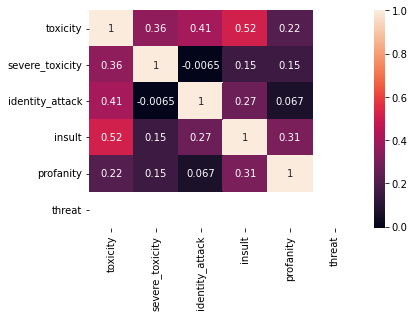
\includegraphics[scale=0.7]{reporting/latex/heatmap-label-corr.png}
\end{figure*}




\end{document}
